\section*{Ход работы:}
\subsection*{Измерение коэффициента усиления}
После тщательной настройки зеркал измеряем коэффициент усиления лазера --- мерим интенсивноть до усиления на фотодиоде 1 и после усиления на фотодиоде 2. Считаем отношение этих величин при включенном и выключенном лазере, а затем считаем отношение этих двух величин.
    \begin{enumerate}
        \item При включенном лазере: \\
        \centering{
         \begin{tabu} to 1\textwidth{|c|c|c|c|c|}
    \hline
    $X_{max}$ & $X_{min}$ & $Y_{max}$ & $Y_{min}$ & отношение $k$ \\
    \hline    
    140,8 & -67,8 & 61,3 & -24,1 & 2,44 \\
    \hline    
    140,8 & -65,8 & 61,3 & -24,1 & 2,42 \\
    \hline    
    138,8 & -67,8 & 61,3 & -26,1 & 2,36 \\
    \hline
    \end{tabu}
    }
    \[\bar{k_1} = 2.41 \pm 0.04 \]
    
    \item При выключенном лазере: \\
    \centering{
         \begin{tabu} to 1\textwidth{|c|c|c|c|c|}
    \hline
    $X_{max}$ & $X_{min}$ & $Y_{max}$ & $Y_{min}$ & отношение $k$ \\
    \hline    
    132,8 & -63,8 & 55,4 & -26,1 & 2,41 \\
    \hline    
    128,9 & -67,8 & 53,4 & -26,1 & 2,47 \\
    \hline    
    138,9 & -71,8 & 55,4 & -28,1 & 2,52 \\
    \hline
    134,8 & -63,8 & 57,4 & -24,1 & 2,44 \\
    \hline
    \end{tabu}
    }
    \[\bar{k_2} = 2.46 \pm 0.05 \]
    
    \item Итоговый коэффициент усиления:
    \[ k = 1.02 \pm 0.03 \]
    \end{enumerate}
    
\subsection*{Проверка поляризации излучения}    
Излучение, генерируемое лазером в теории должно быть поляризованным. Для проверки этого можно пропускать луч через поляризатор и наблюдать за изменением интенсивности пучка после прохода через поляризатор при его повороте. Если излучение поляризовано, то должна получится синусоида.
\centering{
\begin{tabu} to 1\textwidth{|c|c|c|c|c|c|c|}
    \hline
    $\varphi$ & $I_1$ & $I_2$ & $I_3$ & $I_4$ & $I_5$ & $\bar{I}$ \\
    \hline   
    0 & 40,63 & 41,64 & 41,39 & 35,1 & 37,61 & 39,274 \\
    \hline
    20 & 45,87 & 40,75 & 40,45 & 43,29 & 40,92 & 42,256 \\
    \hline
    40 & 62,41 & 62,72 & 63,93 & 63,5 & 59,64 & 62,44 \\
    \hline
    60 & 92,3 & 94,2 & 94,01 & 93,75 & 91,29 & 93,11 \\
    \hline
    80 & 109,92 & 108,22 & 116,61 & 111,63 & 111,1 & 111,496 \\
    \hline
    100 & 103,46 & 107,3 & 114,81 & 108,44 & 107,56 & 108,314 \\
    \hline
    120 & 82,78 & 81,57 & 81,48 & 80,02 & 82,9 & 81,75 \\
    \hline
    140 & 51,49 & 59,44 & 50,92 & 50,13 & 49,53 & 52,302 \\
    \hline
    160 & 35,63 & 39,23 & 41,64 & 37,17 & 39,73 & 38,68 \\
    \hline
    180 & 37,26 & 31,78 & 34,57 & 32,14 & 33,01 & 33,752 \\
    \hline
    200 & 41,58 & 40,28 & 38,58 & 37,18 & 41,78 & 39,88 \\
    \hline
    220 & 60,23 & 60,29 & 61,01 & 61,01 & 62,54 & 61,016 \\
    \hline
    240 & 92,91 & 89,47 & 91,77 & 91,07 & 97,06 & 92,456 \\
    \hline
    260 & 108,64 & 115,57 & 107,98 & 108,83 & 109,92 & 110,188 \\
    \hline
    280 & 113,39 & 107,73 & 114,86 & 113,21 & 111,68 & 112,174 \\
    \hline
    300 & 90,22 & 83,76 & 86,26 & 88,39 & 86,06 & 86,938 \\
    \hline
    320 & 53,13 & 53,62 & 55,49 & 52,72 & 55,94 & 54,18 \\
    \hline
    340 & 32,34 & 36,1 & 35,32 & 42,36 & 41,65 & 37,554\\ 
    \hline
    \end{tabu}
    }
    \\
    
    Тогда график зависимости интенсивности света от угла поворота поляризатора выглядит следующим образом:
    \begin{figure}[h!]
        \noindent\centering{
            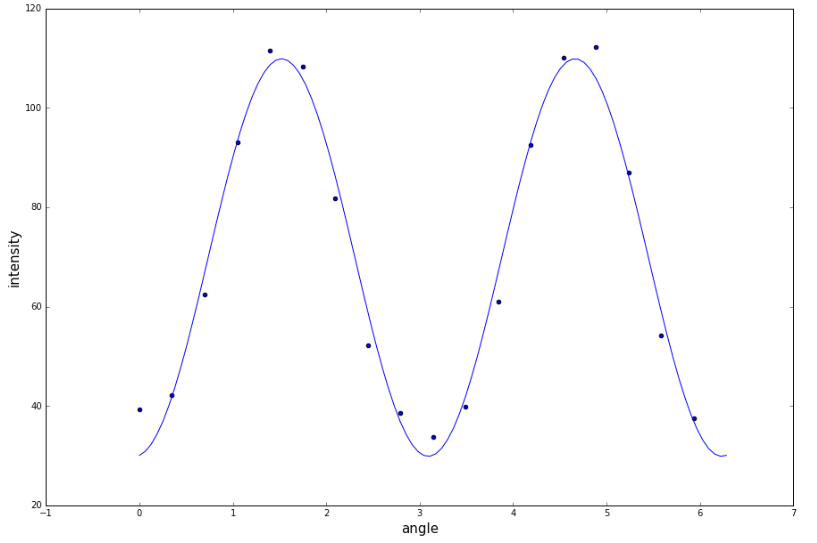
\includegraphics[height = 10cm]{030.png}
        }
        \caption{Синусоида: $y = 40 \sin{(2x + 0.1)} + 70$}
    \end{figure}
    \newpage
    График хорошо аппроксимируется синусоидой, как и ожидалось.